\newpage
\section{Otimização do perfil}

O problema de otimização resolvido nesta seção minimiza o coeficiente de
arrasto do perfil na condição de projeto, tendo como variáveis os
coeficientes CST do intradorso e do extradorso e o ângulo de ataque, e como
restrições a sustentação de projeto e a espessura mínima. Formalmente, o
problema de otimização é enunciado como:

\begin{equation*}
\begin{array}{@{}l@{\qquad}l@{}}
\text{min}    & c_d(\vec{x}) \\[1.4ex]
\text{w.r.t.} & \vec{x} = \begin{bmatrix} A_l & A_u & \alpha \end{bmatrix} \\[1.4ex]
\text{s.t.}   & c_\ell = c_{\ell,\mathrm{ref}} \\[1.0ex]
              & (t/c)_{\max} \ge (t/c)_{\mathrm{ref}} \\[1.0ex]
              & t_{\mathrm{BF}} \le 0{,}01\,c \\[1.0ex]
              & t_{01}/\sqrt{(t/c)_{\max}} \ge 0{,}0938 \\[1.0ex]
              & A_{l,\mathrm{lower}} \preceq A_l \preceq A_{l,\mathrm{upper}} \\[1.0ex]
              & A_{u,\mathrm{lower}} \preceq A_u \preceq A_{u,\mathrm{upper}}
\end{array}
\end{equation*}
\par\medskip

Os valores de referência são os da Tabela~\ref{tab:ref_section}:
$c_{\ell,\mathrm{ref}} = 0{,}7319$ e $(t/c)_{\mathrm{ref}} = 0{,}1772$. Os
batentes seguem o roteiro, $A_{l} \in [-1;\,-0{,}05]$ e
$A_{u} \in [0{,}05;\,1]$, e o ângulo de ataque foi limitado a
$\alpha \in [-3^\circ;\,9^\circ]$. Às restrições do roteiro somaram-se duas:
a espessura do bordo de fuga limitada a $1\%$ da corda ($t_{\mathrm{BF}}$),
que evita bordos de fuga espessos sem função aerodinâmica, e uma restrição
\emph{substituta} de sustentação máxima subsônica,
$t_{01}/\sqrt{(t/c)_{\max}} \ge 0{,}0938$, em que $t_{01}$ é a espessura do
perfil em $x/c = 0{,}01$. Essa métrica de ``afiamento do nariz'' foi
calibrada contra um DOE de 256 perfis analisados no Xfoil e é o descritor
geométrico diferenciável que melhor prevê o $c_{\ell,\max}$. O limiar
$0{,}0938$ corresponde a $c_{\ell,\max} \ge 1{,}80$, valor assumido para
\texttt{clmax\_w} no dimensionamento da aeronave. A Seção~7 mostra o que
acontece sem ela.

O ponto de partida é o NACA~1411 reescalado da Seção~3 e o otimizador é o
SLSQP, com gradientes de $c_\ell$ e $c_d$ calculados pelo método adjunto e
tolerância \texttt{ftol} $= 10^{-5}$. O valor fica acima do piso de
ruído do solver Euler ($1{,}5\times10^{-5}$ em $c_d$, aferido repetindo a
mesma avaliação em malhas perturbadas), pois uma tolerância mais apertada
apenas queimaria avaliações perseguindo ruído numérico.

\begin{table}[H]
\centering
\caption{Dados dos aerofólios da seção de referência.}\label{tab:airfoils_opt}
\renewcommand{\arraystretch}{1.2}
\begin{tabular}{lccl}
\toprule
Parâmetro & NACA 1411 reescalado & Otimizado & Descrição \\
\midrule
$A_{l1}$        & $-0{,}24377$ & $-0{,}18114$ & Parâmetro CST do intradorso \\
$A_{l2}$        & $-0{,}19091$ & $-0{,}39565$ & Parâmetro CST do intradorso \\
$A_{l3}$        & $-0{,}17769$ & $-0{,}13208$ & Parâmetro CST do intradorso \\
$A_{l4}$        & $-0{,}19286$ & $-0{,}05000$ & Parâmetro CST do intradorso \\
$A_{u1}$        & $0{,}25629$  & $0{,}21597$  & Parâmetro CST do extradorso \\
$A_{u2}$        & $0{,}27111$  & $0{,}06141$  & Parâmetro CST do extradorso \\
$A_{u3}$        & $0{,}21590$  & $0{,}44268$  & Parâmetro CST do extradorso \\
$A_{u4}$        & $0{,}26965$  & $0{,}14103$  & Parâmetro CST do extradorso \\
$\alpha$        & $3{,}567$    & $2{,}389$    & Ângulo de ataque [graus] \\
$c_\ell$        & $0{,}7319$   & $0{,}7319$   & Coeficiente de sustentação \\
$c_d$           & $0{,}06705$  & $0{,}01164$  & Coeficiente de arrasto \\
$c_m$           & $-0{,}0680$  & $-0{,}0970$  & Coeficiente de momento \\
$(t/c)_{\max}$  & $0{,}1772$   & $0{,}1772$   & Espessura máxima \\
$x_{t/c,\max}$  & $0{,}296$    & $0{,}364$    & Posição da espessura máxima \\
$(h/c)_{\max}$  & $0{,}0101$   & $-0{,}0152$  & Arqueamento máximo \\
$x_{h/c,\max}$  & $0{,}418$    & $0{,}247$    & Posição do arqueamento máximo \\
\bottomrule
\end{tabular}
\end{table}

A otimização convergiu em 19 avaliações do Euler, em 20,6~minutos. Na
comparação justa, com os dois perfis na \emph{mesma} sustentação de
projeto, o arrasto caiu de $c_d = 0{,}06705$ para
$c_d = 0{,}01164$, uma redução de $\mathbf{82{,}6\%}$. A
Figura~\ref{fig:opt_hist} mostra o histórico: a queda grande acontece nas
primeiras $\sim$8 avaliações, quando o otimizador desmonta o choque forte
do perfil de partida. O restante é ajuste fino dentro do poço.

Quanto às restrições, todas as três não-triviais terminaram
\textbf{ativas}: a igualdade de sustentação (por construção), a espessura
mínima ($(t/c)_{\max} = 0{,}17720$, exatamente no limite, sinal de que o
otimizador afinaria o perfil se pudesse, pois espessura custa arrasto de
onda) e a substituta de $c_{\ell,\max}$ ($0{,}09382$, exatamente sobre o
limiar, sinal de que o otimizador afiaria o nariz se pudesse, ao custo do
estol). Um batente também terminou ativo, o $A_{l4} = -0{,}05$, coeficiente
que controla o côncavo do intradorso traseiro (\emph{cusp}). O roteiro o limita
justamente para conter o $c_m$, e a Seção~7 quantifica essa troca.

Duas verificações dão confiança de que esse é, de fato, o ótimo do
problema, e não um acidente numérico. Primeiro, \emph{multistart}: seis
pontos de partida geometricamente distintos, com $c_d$ inicial variando por
um fator 2,5, convergiram todos para o mesmo ponto, com espalhamento de
$2{,}6\times10^{-6}$ em $c_d$, seis vezes menor que o piso de ruído do
solver. Segundo, cortes unidimensionais em torno do ótimo: deslocando cada
coeficiente CST de até $\pm0{,}06$ com o $c_\ell$ re-trimado, nenhuma das 41
direções avaliadas (de 48 planejadas, 7 caem fora dos batentes) reduz o
arrasto sem violar uma restrição. A espessura barra 24 direções, a
substituta de $c_{\ell,\max}$ barra 13 (quatro por ambas), uma sai do alvo
de $c_\ell$ e nas 7 restantes o arrasto simplesmente piora. O perfil obtido
é o mínimo de arrasto possível dada a espessura estrutural que a asa exige.

\begin{figure}[H]
    \centering
    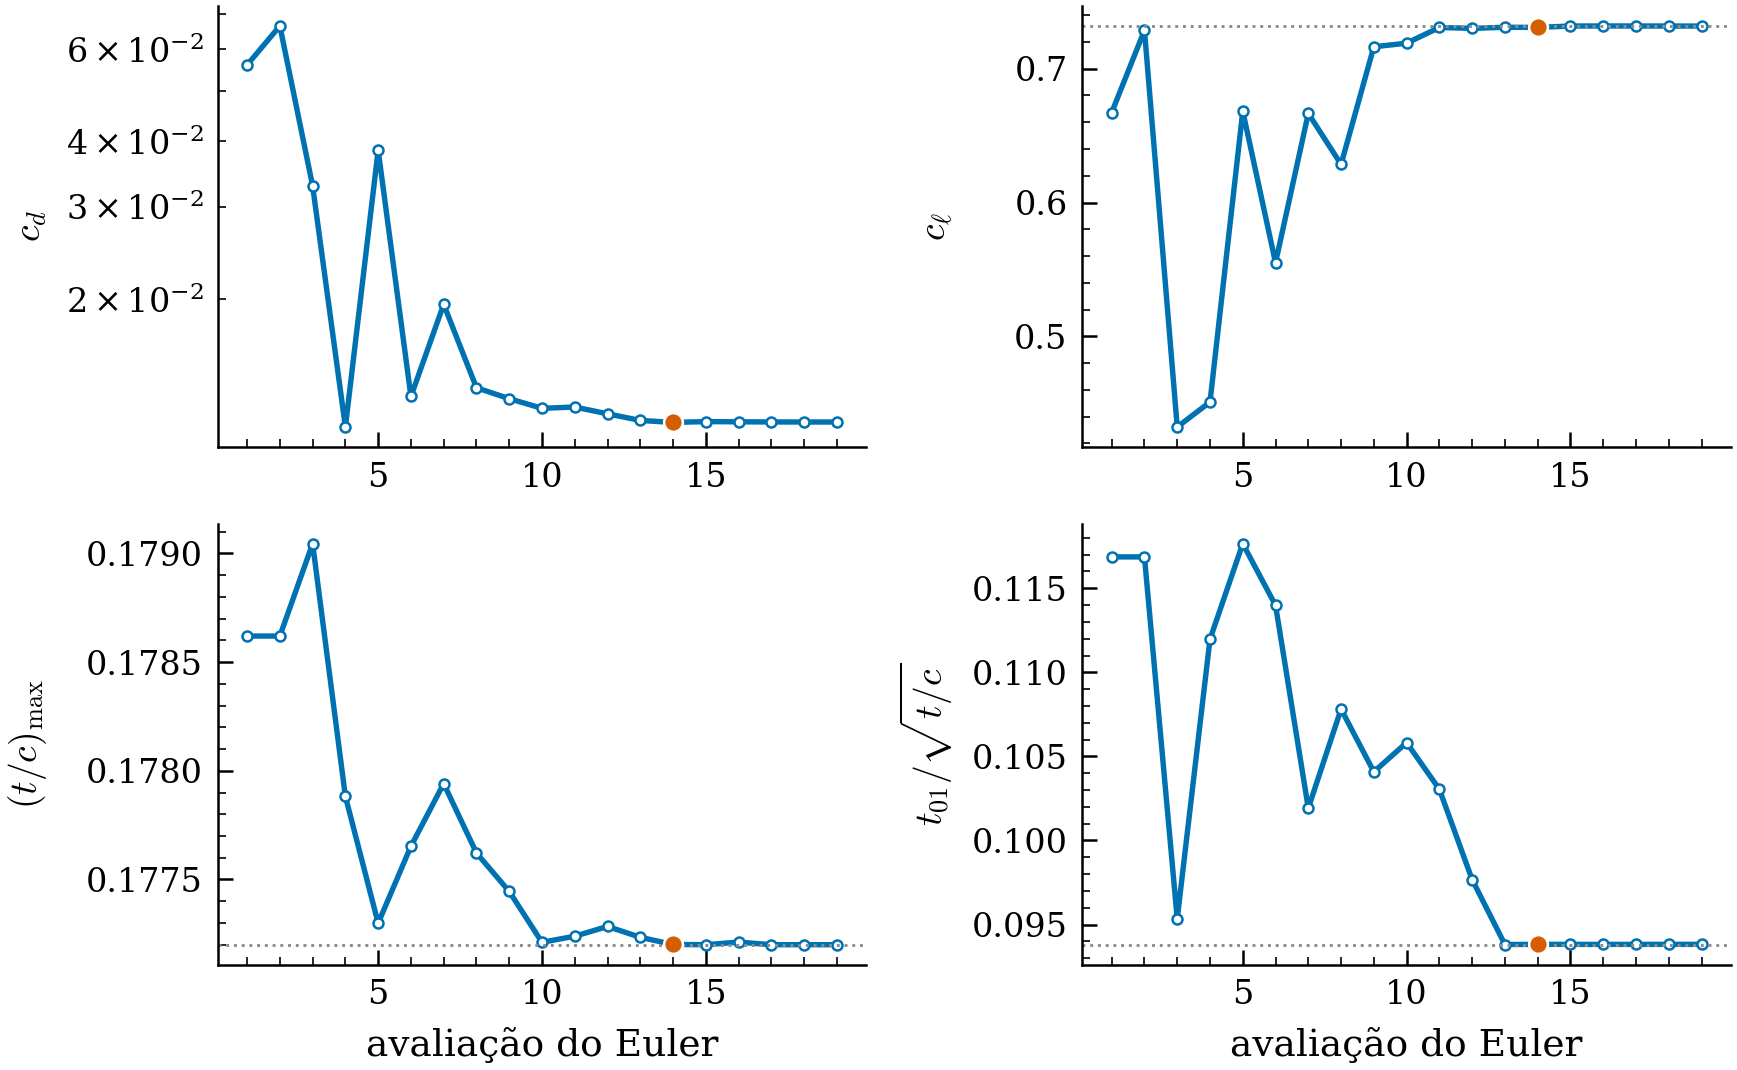
\includegraphics[width=0.9\textwidth]{images/04_otimizacao/historico_convergencia.png}
    \caption{Histórico de convergência da otimização: $c_d$ (escala
    logarítmica), $c_\ell$, $(t/c)_{\max}$ e a substituta de
    $c_{\ell,\max}$ ao longo das avaliações do Euler. As linhas tracejadas
    marcam o alvo de sustentação e os limites das restrições. Note
    $(t/c)_{\max}$ e a substituta terminando sobre os respectivos limites
    (restrições ativas).}\label{fig:opt_hist}
\end{figure}
